\documentclass{article}
\PassOptionsToPackage{numbers,compress}{natbib}
\usepackage[preprint]{neurips_2026}

\usepackage[utf8]{inputenc}
\usepackage[T1]{fontenc}
\usepackage{hyperref}
\usepackage{url}
\usepackage{booktabs}
\usepackage{amsfonts}
\usepackage{amsmath}
\usepackage{microtype}
\usepackage{xcolor}
\usepackage{graphicx}

% This is an ES 678 course paper, not a conference submission.
\makeatletter
\renewcommand{\@noticestring}{ES 678 Course Project}
\makeatother

\title{NationPulse: Measuring AI Bias in Economic Assessment of Developing Countries}

\author{%
  Jay Prafulkumar Joshi \\
  Roll Number 26210062 \\
  ES 678 \\
  Indian Institute of Technology Gandhinagar
}

\begin{document}
\maketitle

\begin{abstract}
Can a local large language model (LLM) judge a country's economy and suggest how to improve it as well as a small explainable model? We compare XGBoost with SHAP explanations against the Mistral 7B LLM on 52 countries, using seven World Bank and IMF indicators from 2014 to 2023. Neither system judges the other. Both are checked against the real score, the speed of change countries have achieved, economic advice, and computing cost. On countries it never saw in training, XGBoost is 9.1 points off on a 0 to 100 scale. The LLM is 17.8 points off, worse than a simple linear regression (13.3). It gives most countries a middle score, so it rates low-income countries 34 points too high. Its growth plans always follow economic advice, while XGBoost's own plans break it in 30 of 51 countries. Overall, XGBoost does better on 8 measures and the LLM on 2.
\end{abstract}

\section{Problem and Motivation}
People now ask LLMs for economic advice, but nobody can see how an LLM reaches its answer. An explainable model shows its reasoning. We ask in which parts of judging and improving an economy each kind of system does better, and whether either is biased against developing countries. Each row of data is one country in one year, described by seven indicators. The target is an economic score, the log of GDP per capita scaled from 0 to 100. Each system scores a country from the same year's indicators, and we score the year 2023. Each system also suggests how the indicators should change to raise the score by 10 points within 5 years. The data can show which indicators go together with higher income. It cannot show which policy causes growth.

\textbf{Contributions.} First, we compare an explainable model and an LLM as equal competitors, with neutral checks instead of using one system to judge the other. Second, we test both systems on countries they never saw, and show how much an unfair test would have flattered the explainable model. Third, we compare growth plans from both systems with checks that need no model. Fourth, we report the explainable model's own flaws, such as recommending more government debt. Fifth, we add the environmental cost of each system to the comparison.

\section{Data and Preparation}
\textbf{Sources.} The World Bank \citep{worldbank2026wdi} gives GDP per capita, inflation, unemployment, foreign investment, trade, life expectancy and education spending, collected from the IMF, ILO, UN, UNESCO and national offices. Government debt comes from the IMF \citep{imf2026weo}, because the World Bank had no debt figures for 21 of our first 41 countries. The IMF figure covers all levels of government, so it is higher than central government debt in federal countries such as India. We use 52 countries from all four income groups (4 low, 14 lower-middle, 19 upper-middle, 15 high) for 2014 to 2023, which gives 520 rows. The data may be shared with credit, but the IMF data needs permission for commercial use.

\textbf{Checks and preparation.} The \texttt{wbgapi} download tool stopped working, so we used the World Bank's basic web address, and we fixed one mistyped indicator code. Before filling, inflation had 4 missing values, trade 11 and education spending 67. Missing values were filled from the same country's other years only, so no information passes between training and test countries. Three gaps remain (trade for Nigeria and Jordan, education for Egypt). XGBoost works with gaps, and the linear baseline fills them with training medians. Only the 0 to 100 scaling uses all rows, and it is the same fixed scale for both systems.

\section{Methods}
\textbf{Target.} For country $i$ with GDP per capita $g_i$, the score is $s_i = 100\,(\log g_i - m)/(M - m)$, where $m$ and $M$ are the lowest and highest $\log g$ in the data.

\textbf{Baselines.} The first baseline always predicts the average score of the training countries. The second is a linear regression on the seven indicators.

\textbf{System 1, XGBoost and SHAP.} XGBoost \citep{chen2016xgboost} adds up many small decision trees, $\hat s(x)=\sum_k f_k(x)$. Training makes $\sum_i (s_i-\hat s_i)^2+\sum_k(\gamma T_k+\tfrac12\lambda\lVert w_k\rVert^2)$ small, where tree $k$ has $T_k$ leaves with values $w_k$, and the second part keeps the trees simple. We use 200 trees of depth 3, fixed before testing. SHAP \citep{lundberg2017unified,lundberg2020local} splits each score into one part per indicator, $\hat s(x)=\phi_0+\sum_{j=1}^{7}\phi_j(x)$, so we can see how much each indicator $j$ adds or removes. A conformal method \citep{vovk2005algorithmic,lei2018distribution} gives a 95\% range around each score.

\textbf{System 2, the LLM.} Mistral 7B \citep{jiang2023mistral} runs on the laptop through Ollama at temperature 0. It gets the same seven numbers and gives a score and a weight for each indicator. The prompt shows empty slots, not example numbers, which biased the answers (Section~\ref{sec:depth}).

\textbf{Growth plans.} The target is 10 more points in $T=5$ years. For each indicator $j$, the limit $L_j$ is how fast the fastest 10\% of countries changed it per year from 2014 to 2023. System 1 searches step by step, each round moving one indicator by up to $T L_j$ where the predicted score rises most per step. It runs once allowing only the direction economists recommend (for example lower unemployment) and once with no rule, to show the model's own choice. The LLM gives a target value, a priority and a short reason for each indicator.

\section{Evaluation Design}
No system judges the other. Scores are compared with the real score $s_i$. The LLM never sees $s_i$, so for fairness each country is scored by an XGBoost or baseline model trained on the other 51 countries. No settings were tuned, so no test information was used to choose the models. We measure the average error $\tfrac1n\sum_i|\hat s_i-s_i|$, how well each system ranks the countries (Spearman correlation with $s_i$), and the average error $b_g$ in each income group and region, comparing the worst group. We also measure how much the LLM's score changes when the question is reworded or written as sentences. For the 95\% range, a model trained on 70\% of countries gives the score plus or minus $\hat q$, the $\lceil 0.95(n+1)\rceil/n$ quantile of absolute errors on the other 30\%. Only a competitor model could say whether a plan reaches its target, so plans are checked in two ways that need no model. Realism is the share of changes no bigger than $T L_j$ and inside the range seen in the data. Direction is the share of changes that follow economic advice. Cost is run time times the processor's 15\,W rating, with 0.727\,kg of carbon dioxide \citep{cea2024baseline} and 3.5 litres of water per kWh.

\section{Results and Error Analysis}

\begin{table}[t]
\centering
\footnotesize
\setlength{\tabcolsep}{4pt}
\begin{tabular}{p{4.9cm}p{3.3cm}p{3.0cm}l}
\toprule
Measure & XGBoost + SHAP & LLM & Better \\
\midrule
\multicolumn{4}{l}{\emph{Scoring countries}} \\
Average error (points) & \textbf{9.1} & 17.8 & XGBoost \\
Baselines, average error & \multicolumn{2}{l}{guess the average 21.8, linear regression 13.3} & for scale \\
Ranking correlation & \textbf{0.87} & 0.63 & XGBoost \\
Error in the worst income group & \textbf{8.4} & 33.6 & XGBoost \\
Error in the worst region & \textbf{14.6} & 28.6 & XGBoost \\
Change when the question is reworded & \textbf{0} & 13.8 & XGBoost \\
Gives a 95\% range & \textbf{yes, $\pm$22.9} & no & XGBoost \\
Change when numbers become sentences & cannot be tested & 8.4 & no winner \\
Agreement on which indicators matter & \multicolumn{2}{l}{$-0.19$ (one shared value)} & no winner \\
Countries scored & 100\% & 100\% & tie \\
\midrule
\multicolumn{4}{l}{\emph{Growth plans}} \\
Realistic changes (\%) & \textbf{100} (by design) & 65 & XGBoost \\
Changes that follow economic advice (\%) & 74 (no rule) & \textbf{100} & LLM \\
Plans with a change against economic advice & 30 of 51 (no rule) & \textbf{0} & LLM \\
Countries with a plan & 100\% & 100\% & tie \\
Indicators changed per plan & 2.0 & 6.9 & no winner \\
How the plan is explained & SHAP gain per indicator & priority and reason & no winner \\
\midrule
\multicolumn{4}{l}{\emph{Environmental cost (52 countries, estimated)}} \\
Time, energy, carbon dioxide, water & \textbf{4.1\,s, 0.017\,Wh, 0.012\,g, 0.06\,ml} & 163\,min, 40.8\,Wh, 29.7\,g, 143\,ml & XGBoost \\
\bottomrule
\end{tabular}
\caption{The final scoreboard, as in the dashboard. Errors are in points on the 0 to 100 scale, for countries each model did not train on. Bold marks the better system. XGBoost does better on 8 measures and the LLM on 2. Two are ties and four have no winner.}
\label{tab:scoreboard}
\end{table}

\begin{figure}[t]
\centering
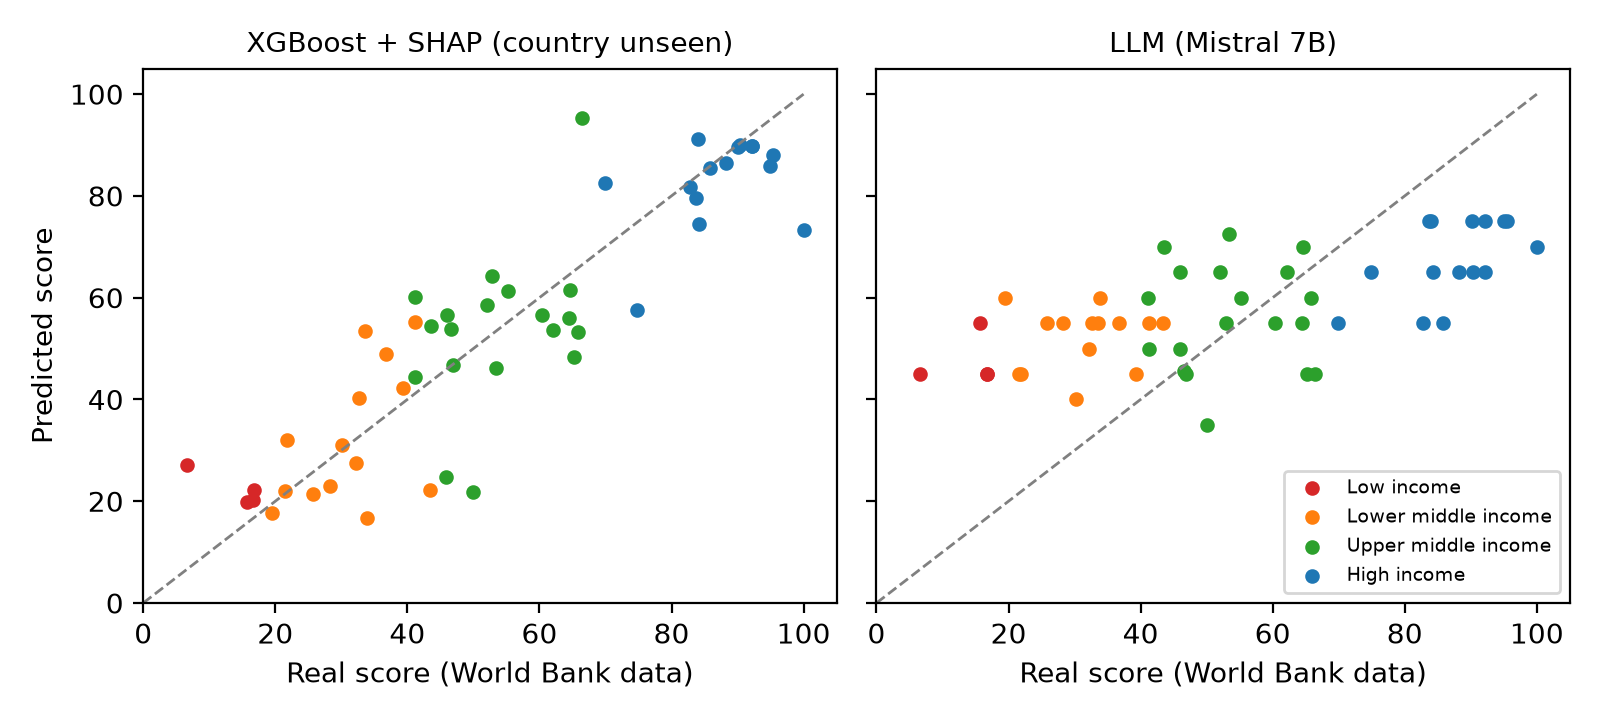
\includegraphics[width=0.75\linewidth]{figures/prediction_scatter.png}
\caption{Each system's score against the real score, one dot per country. Dots on the dashed line are exactly right.}
\label{fig:scatter}
\end{figure}

\textbf{Scoring.} Table~\ref{tab:scoreboard} brings every comparison together. The LLM beats guessing the average but not a linear regression. Figure~\ref{fig:scatter} shows its main problem. All its scores fall between 35 and 75, so poor countries score too high (Tanzania 60 against a real 20) and rich ones too low (Italy 55 against 86). This is the bias against developing countries we set out to measure, but it runs upwards. Its group errors run from 34 points too high for low income to 20 too low for high income, against 8 and 4 for XGBoost. Rewording changed Argentina's score from 45 to 25.5. XGBoost fails differently. It cannot predict above the highest score seen (United States 73 against 100), and values unlike any training country mislead it (Argentina's 133\% inflation, predicted 95 against 66). SHAP finds that life expectancy drives 70\% of XGBoost's scores. The LLM says it weighs unemployment (20\%), inflation (18\%) and debt (17\%) most, and life expectancy only 11\%. The LLM's weights look like textbook advice, while XGBoost leans on one indicator that tracks income closely. With no true answer, neither can be called right.

\textbf{Growth plans.} The LLM always follows economic advice and explains each change, but only 65\% of its changes are realistic. For low-income countries only 36\% are, against 71\% for high-income countries, mostly because it asks for impossible gains in life expectancy (42 times) and education spending (36). XGBoost stays inside the limits by design, and most often changes life expectancy (34 of 51 plans). Without the economics rule it moves an indicator the wrong way in 30 of 51 countries, mostly adding debt (15) or cutting trade (11), because rich countries carry high debt in the data. This happens in 13 of 14 high-income countries, where its plans also rarely reach the target (1 of 14 by its own estimate).

\section{Graduate Depth Analysis}
\label{sec:depth}
\textbf{How much does a fair test change the answer?} Tested on countries it trained on, XGBoost's error is 3.1 and its ranking correlation 0.98. On unseen countries they are 9.1 and 0.87. The first result is three times too good and would have made the gap to the LLM look like 14.7 points instead of 8.7. XGBoost still beats the linear baseline (9.1 against 13.3), so learning curves adds accuracy, but not outside the training range.

\textbf{Uncertainty.} The 95\% range is plus or minus 22.9 points and held the real score for all 16 test countries. At 96\%, 97\%, 98\% and 99\% it grows only to 23.1, 24.3, 25.9 and 26.5. XGBoost can say how unsure it is, and it is quite unsure. The LLM gives no range, though its scores are 17.8 points off on average.

\textbf{Prompt check.} One example number in the prompt (a score of 50) made Mistral give most countries 55 to 70, and empty slots fixed it. With the 13.8-point rewording and 8.4-point sentence effects, this shows the LLM's answer depends on how the question is asked. XGBoost's does not.

\section{Limitations and Conclusion}
The most important limitation is that the score only measures GDP per capita, and XGBoost and SHAP only show which indicators go together with higher income. A plan that raises the predicted score might not raise real income, and the debt result shows why. A stronger claim would need a backtest, where plans are made from 2014 to 2018 data and compared with what countries really achieved by 2023. Other limits are 52 countries, one small LLM that may have memorised GDP figures, checks we designed ourselves, an estimated energy cost, and Mistral not repeating exactly at temperature 0. \textbf{In conclusion}, XGBoost with SHAP is better at scoring countries. It is more accurate, fairer to developing countries and more consistent, states its uncertainty and costs far less. The LLM is better at plans that follow economic advice, but its plans are often unrealistic, especially for poor countries. The two systems fail in different ways.

\section{Reproducibility and AI-Use Disclosure}
The code is at \url{https://github.com/Jay-Joshi-GIT/nationpulse}. This paper shows one figure. The other plots, such as the bar chart of all 52 countries, the SHAP summary plot and the environmental cost chart, are in the \texttt{results} folder of the repository, and its dashboard shows each country's results and plans. The data was downloaded by \texttt{data\_pipeline.py} on 20 October 2026, and \texttt{CREDITS.md} lists every source. The README gives the order of the scripts. All splits use \texttt{random\_state=42}, and the LLM is \texttt{mistral} through Ollama 0.40.6. No passwords, keys or private data are included.

\textbf{AI use.} Claude Code by Anthropic was used to write and debug the code, run the pipeline and draft this paper. Some decisions were made without AI. These were the choice of XGBoost and SHAP as System 1, all data decisions including the use of IMF data for government debt, and the idea of comparing environmental cost. The project began as the strategy planner, and the other comparisons in the dashboard were added while working with the AI. All AI-generated code was checked by hand to do what it should, the dashboard and strategy planner outputs were checked for different countries, and the web page layout was checked. Mistral 7B is the system being studied, not a writing aid.

\small
\bibliographystyle{abbrvnat}
\bibliography{references}

\end{document}
